\documentclass{cmspaper}
\input epsf
\usepackage{graphicx}
\begin{document}

%==============================================================================
% title page for few authors

\begin{titlepage}

% select one of the following and type in the proper number:
%  \cmsnote{2005/000}
  \internalnote{2006/000}
%  \conferencereport{2005/000}
   \date{8 November 2006}

  \title{The CMS Storage Manager}

  \begin{Authlist}
    A.~Afaq, W.~Badgett, K.~Biery, H.~Cheung, J.~Kowalkowski, 
    E.~Sexton-Kennedy
       \Instfoot{fermilab}{Fermilab, Batavia, IL, USA}
    M.~Klute, C.~Paus
       \Instfoot{mit}{MIT, Cambridge, MA, USA}
  \end{Authlist}

% if needed, use the following:
\collaboration{Storage Manager Working Group}
%\collaboration{CMS collaboration}


  \begin{abstract}
    Documentation for the Storage Manager, including the requirements,
    architecture and design, implementation, and a user manual.
  \end{abstract} 

% if needed, use the following:
%\conference{Presented at {\it Physics Rumours}, Coconut Island, April 1, 2005}
%\submitted{Submitted to {\it Physics Rumours}}
%\note{Working version}
  
\end{titlepage}

\setcounter{page}{2}%JPP

%==============================================================================
% title page for many authors
%
%\begin{titlepage}
%  \internalnote{2005/000}
%  \title{CMS Technical Note Template}
%
%  \begin{Authlist}
%    A.~Author\Iref{cern}, B.~Author\Iref{cern}, C.~Author\IAref{cern}{a},
%    D.~Author\IIref{cern}{ieph}, E.~Author\IIAref{cern}{ieph}{b},
%    F.~Author\Iref{ieph}
%  \end{Authlist}
%
%  \Instfoot{cern}{CERN, Geneva, Switzerland}
%  \Instfoot{ieph}{Institute of Experimental Physics, Hepcity, Wonderland}
%  \Anotfoot{a}{On leave from prison}
%  \Anotfoot{b}{Now at the Moon}
%
%  \begin{abstract}
%    This is a template of a CMS paper, written in LaTeX,
%    processed with {\it cmspaper.sty} style.
%    It is based on the {\it cernart.sty} and {\it articlet.sty} styles.
%    There are two versions of the title page.
%    The current one is designed for many authors.
%    The one on the previous page is for few authors.
%    Just delete the one which you do not need.
%  \end{abstract} 
%  
%\end{titlepage}
%
%==============================================================================

\section{Introduction to the Storage Manager}

\section{Use Cases}

\subsection{Use Cases for Data Flow}


\subsection{Use Cases for Event Consumers}



\section{Requirements}

\subsection{Data Flow Requirements}

\subsubsection{Event Rates, Data Bandwidth, and Output Streams}

Include Event Server.

\subsubsection{Scale and Scalability}

\subsubsection{Streamer Service and Data Format and Data Types}
 
\begin{itemize}
\item
input
\item
output
\item
partial data
\item
other types of data (DQM)
\item
conversion
\item
file index
\item
version compatibility
\item
Streamer utilities
\end{itemize}
   
\subsubsection{Book-keeping Requirements}

\subsubsection{Performance, Reliability, and Robustness}

\subsubsection{Status, Monitoring, Statistic}

\subsubsection{Data file management}

interaction with Tier-0, DQM, consumers, express streams

\subsection{Requirements for Event Server and Event Consumers}


\subsubsection{Event Rates, Data Bandwidth}

\subsubsection{Data Format and Dependencies on Software}

 (e.g. curl, not xdaq, etc.)

\subsubsection{Data Access}
 
  (remote, security)

\subsubsection{Data selection}
  
(rare events from all subfarms, etc., lossless/lossy?)

\begin{itemize}
\item
Event selection
\item
Data or branch selection
\end{itemize}

\subsubsection{Performance, Robustness, Reliability}

(impact on logging and SM)

\subsubsection{Status, Monitoring, Statistics}

\subsection{Requirements for Hardware}

\subsubsection{Network}

\subsubsection{Disk Servers}

\subsubsection{Performance and Reliability}

(redundancy, uptime, data integrity, Concurrent RW)


\subsection{Dependencies of the Storage Manager on Framework and External Libraries}

\subsubsection{Streamer output and input services}

\subsubsection{Pool output service}

\subsubsection{API to manage output runs and luminosities, partial data}

\section{Design and Implementation}

\subsection{Architecture}

\subsubsection{Data Flow}

\subsubsection{Current Base Design}

\begin{figure}[hbtp]
  \begin{center}
    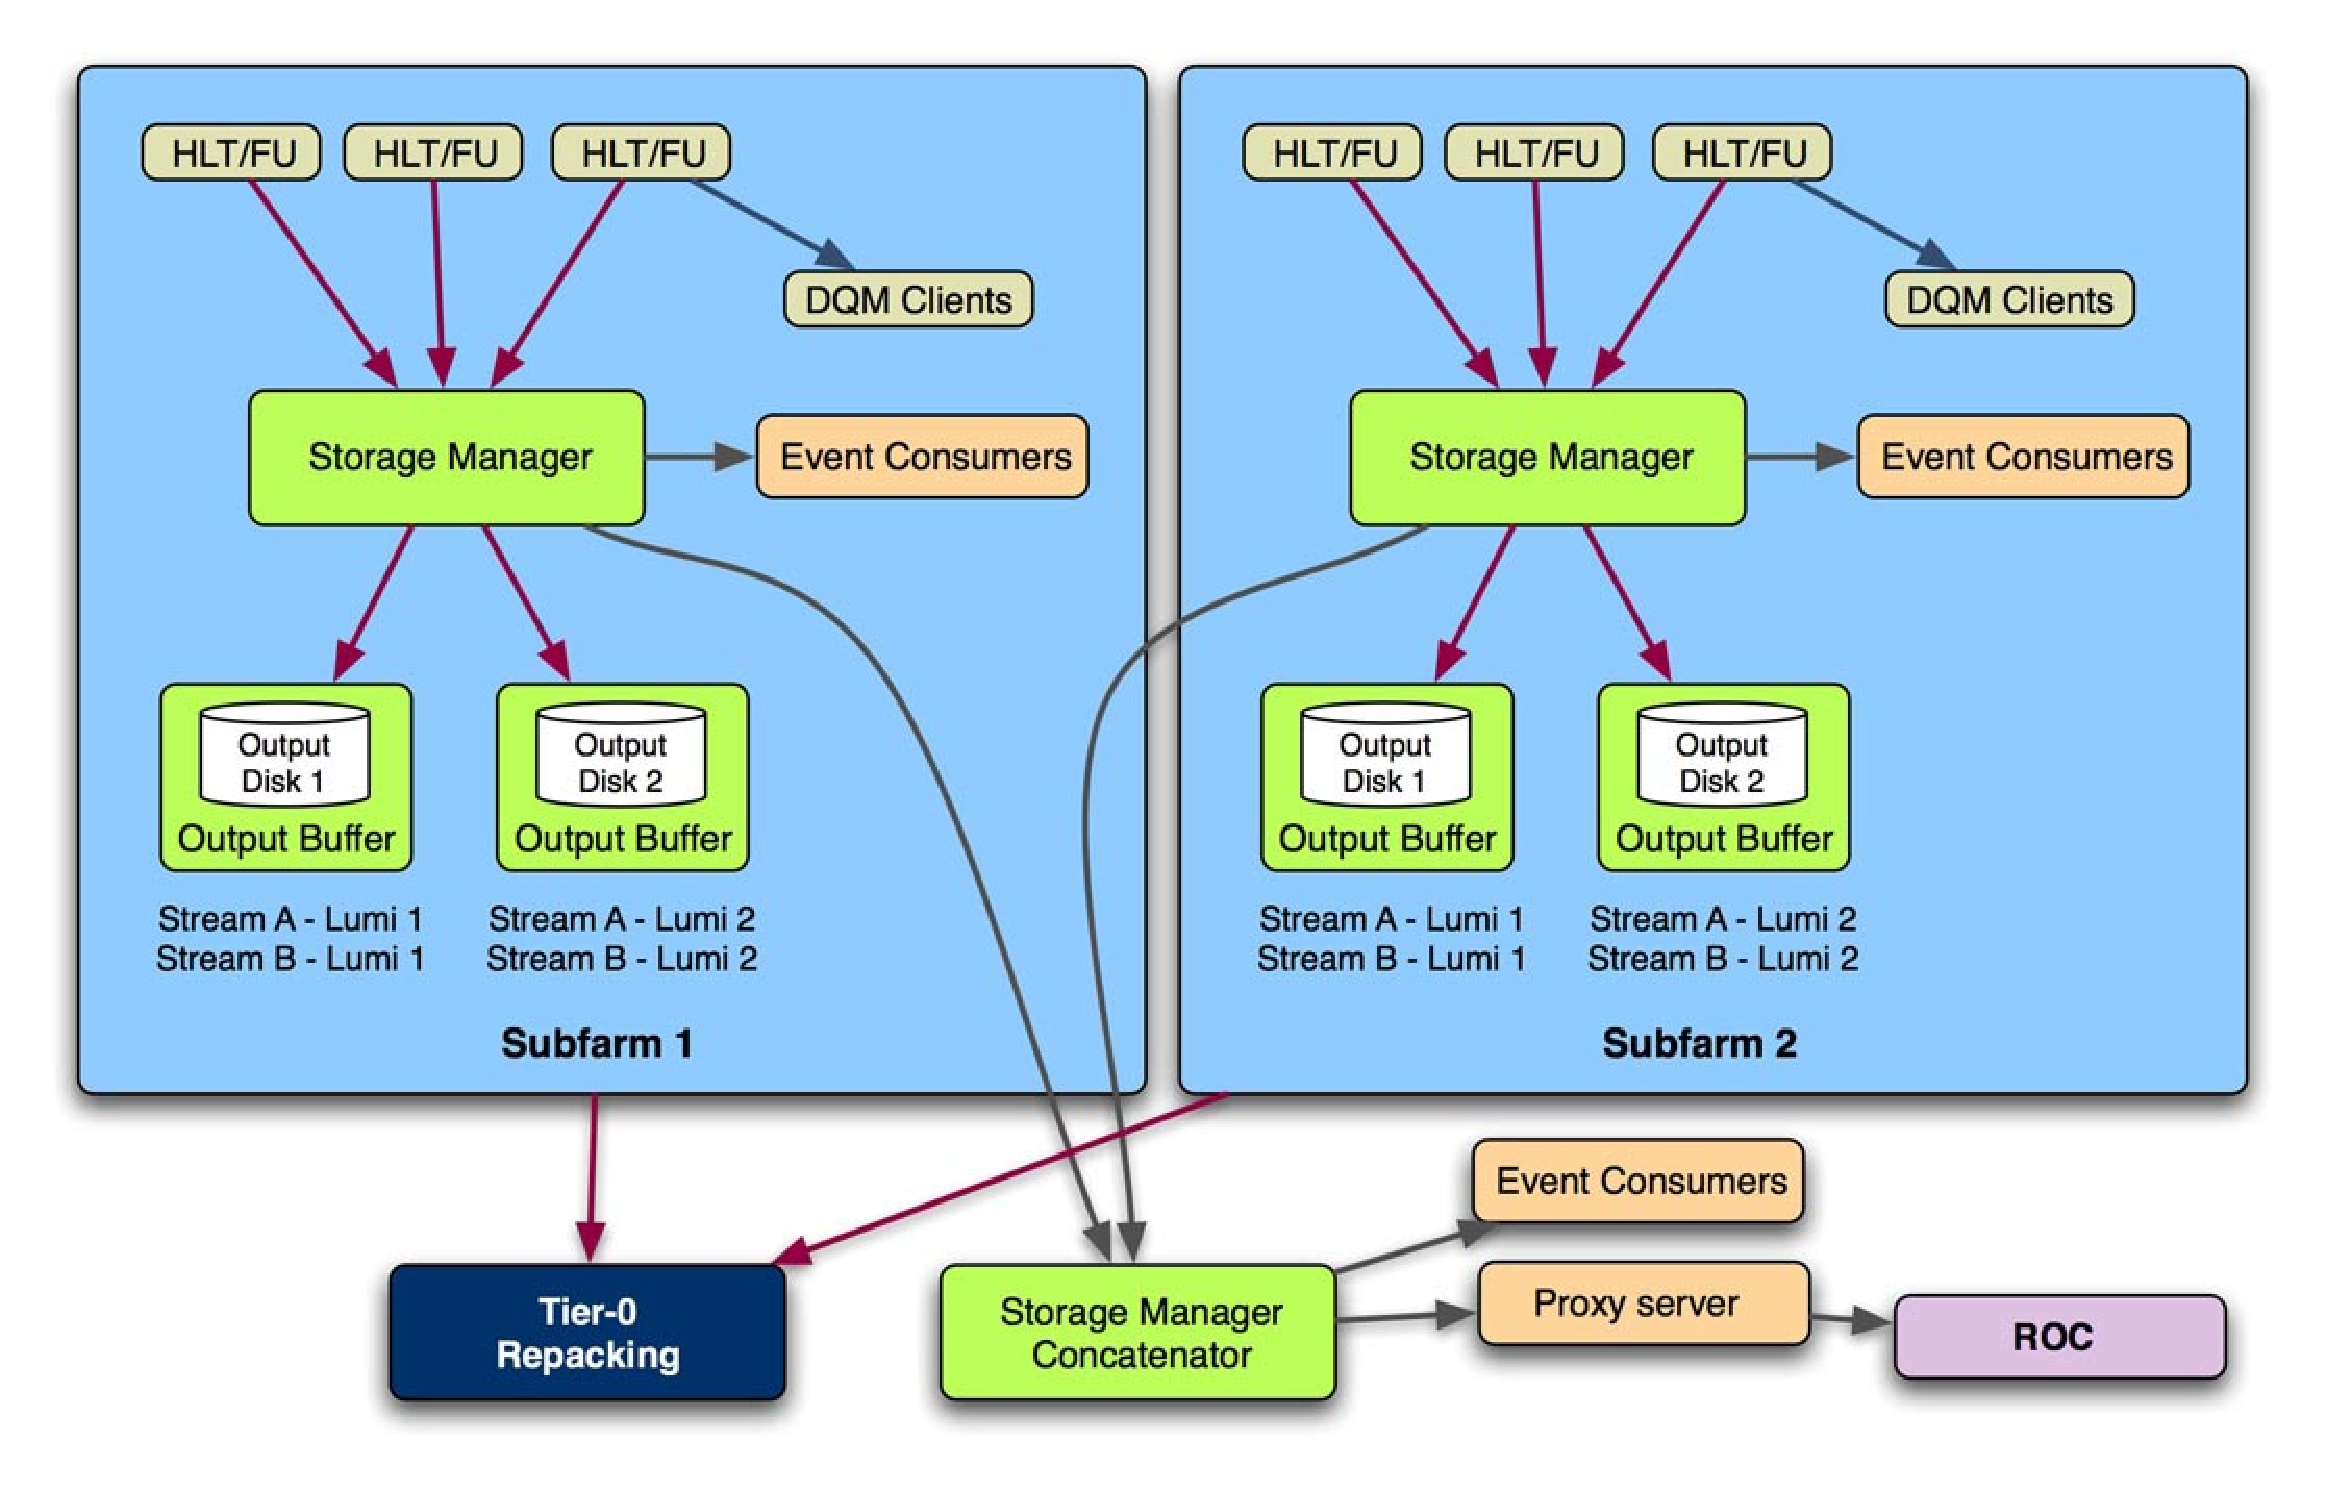
\includegraphics[width=5.5in]{SM_architecture_base.eps}
    \caption{Base design.}
    \label{fig:base_design}
  \end{center}
\end{figure}

\subsubsection{Implementation Details}

\begin{figure}[hbtp]
  \begin{center}
    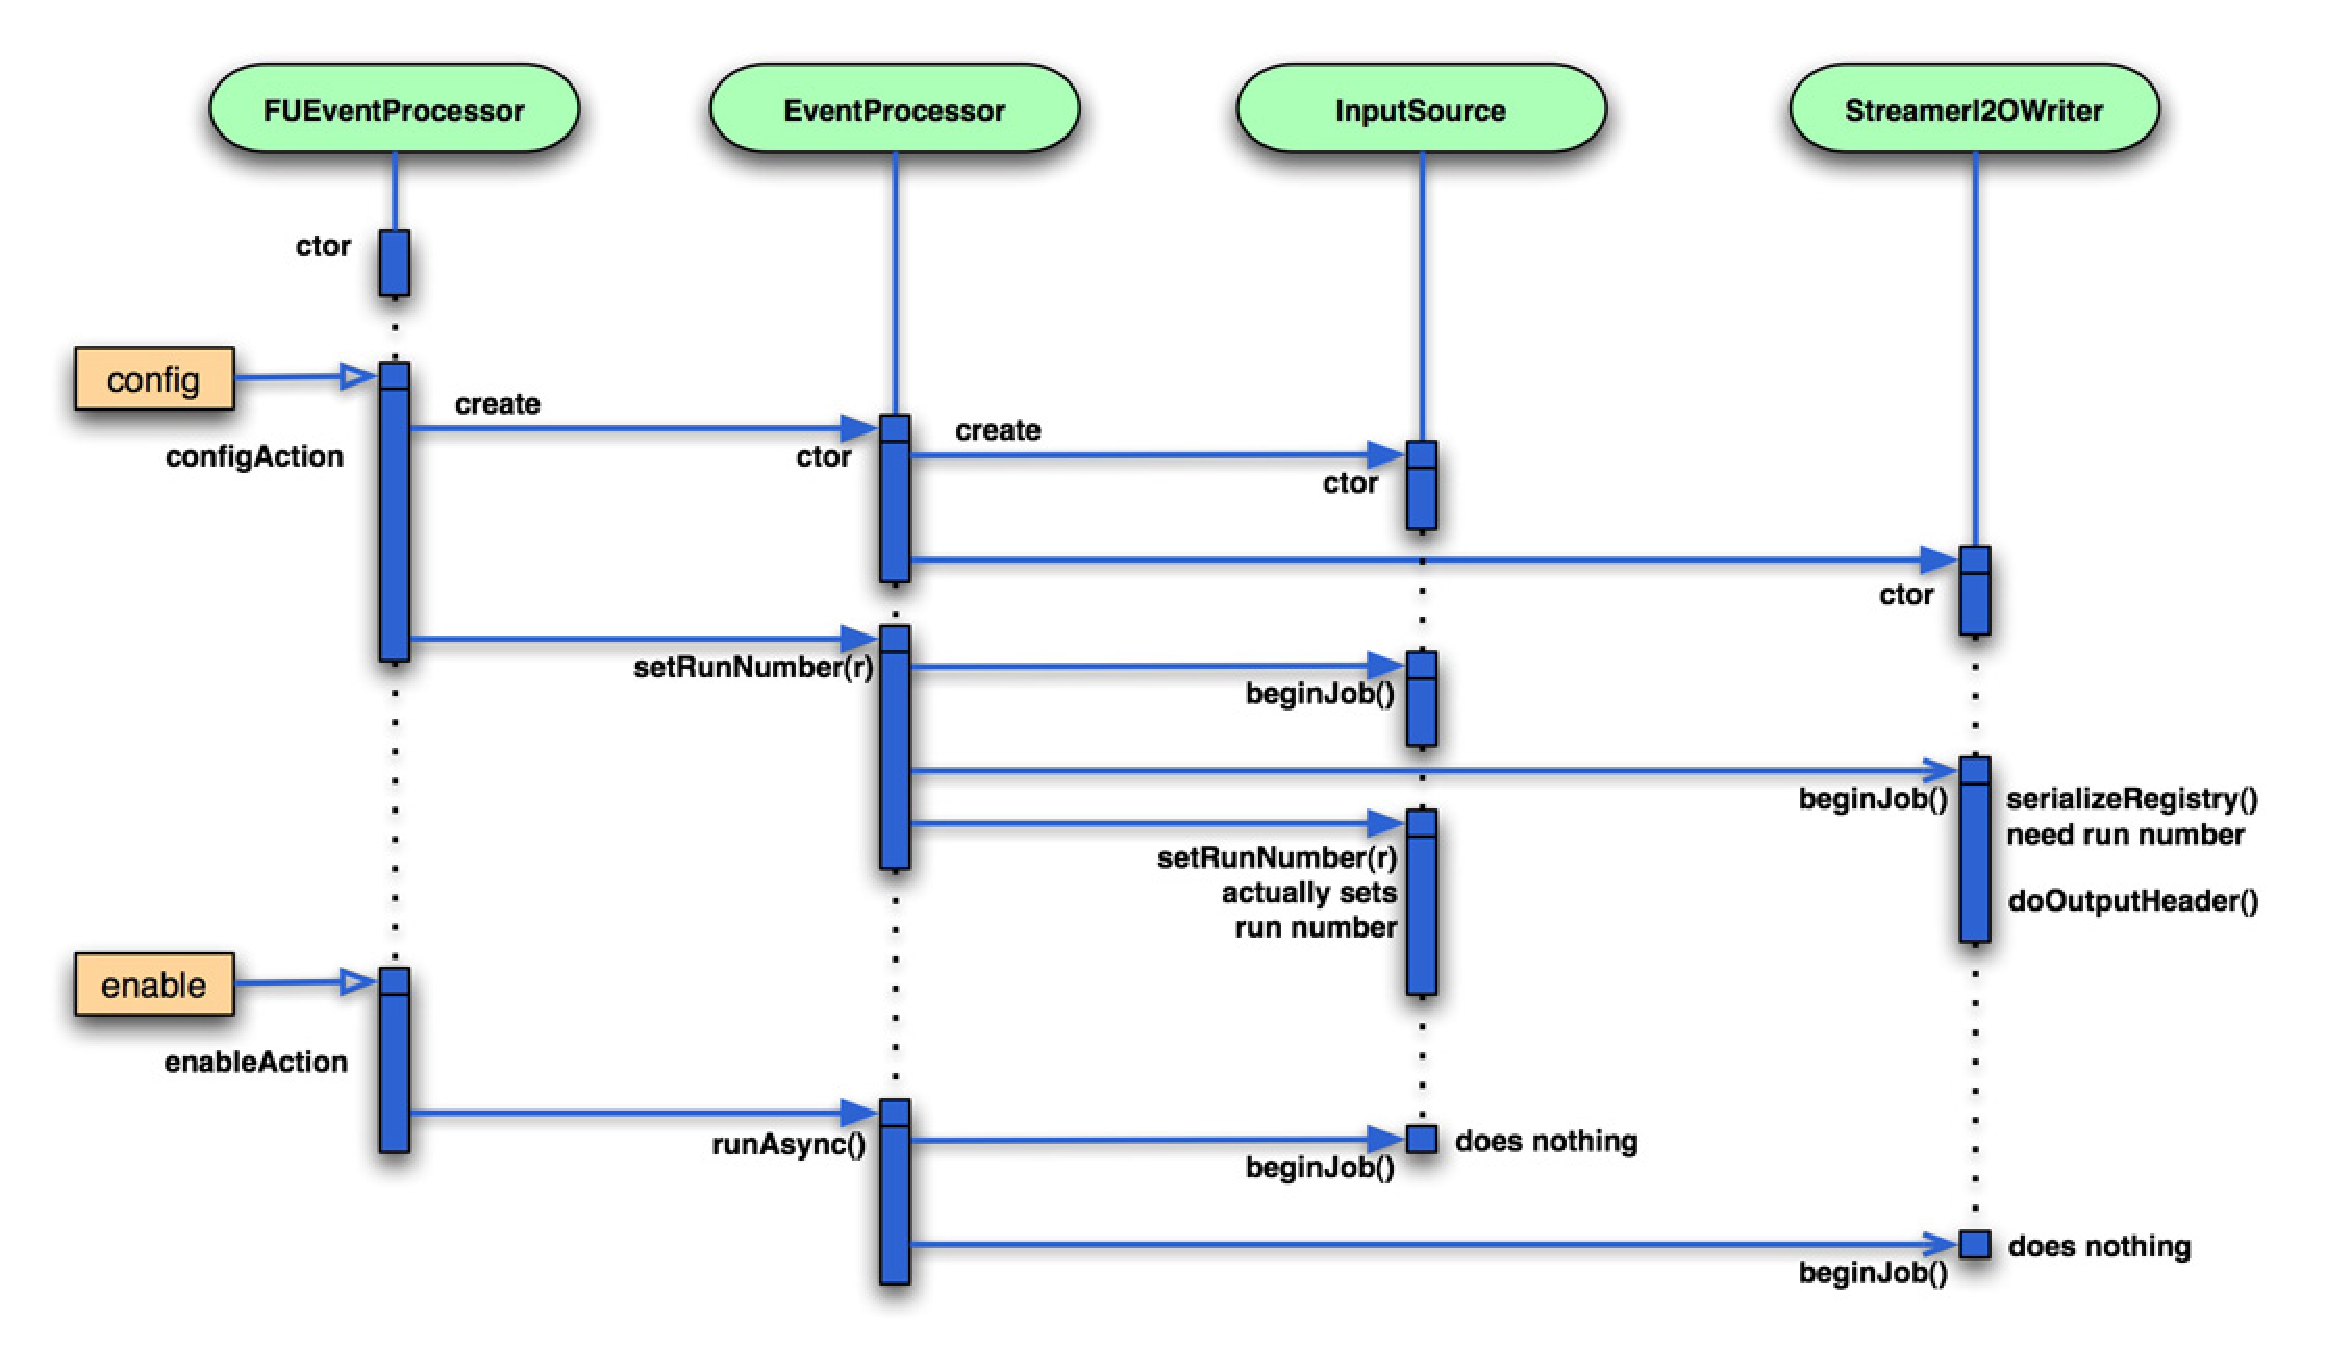
\includegraphics[width=5.5in]{SM_base_code1_prt-2.eps}
    \caption{FUEventProcessor call sequence for setting the run number.}
    \label{fig:base_FUEP_code}
  \end{center}
\end{figure}

\begin{figure}[hbtp]
  \begin{center}
    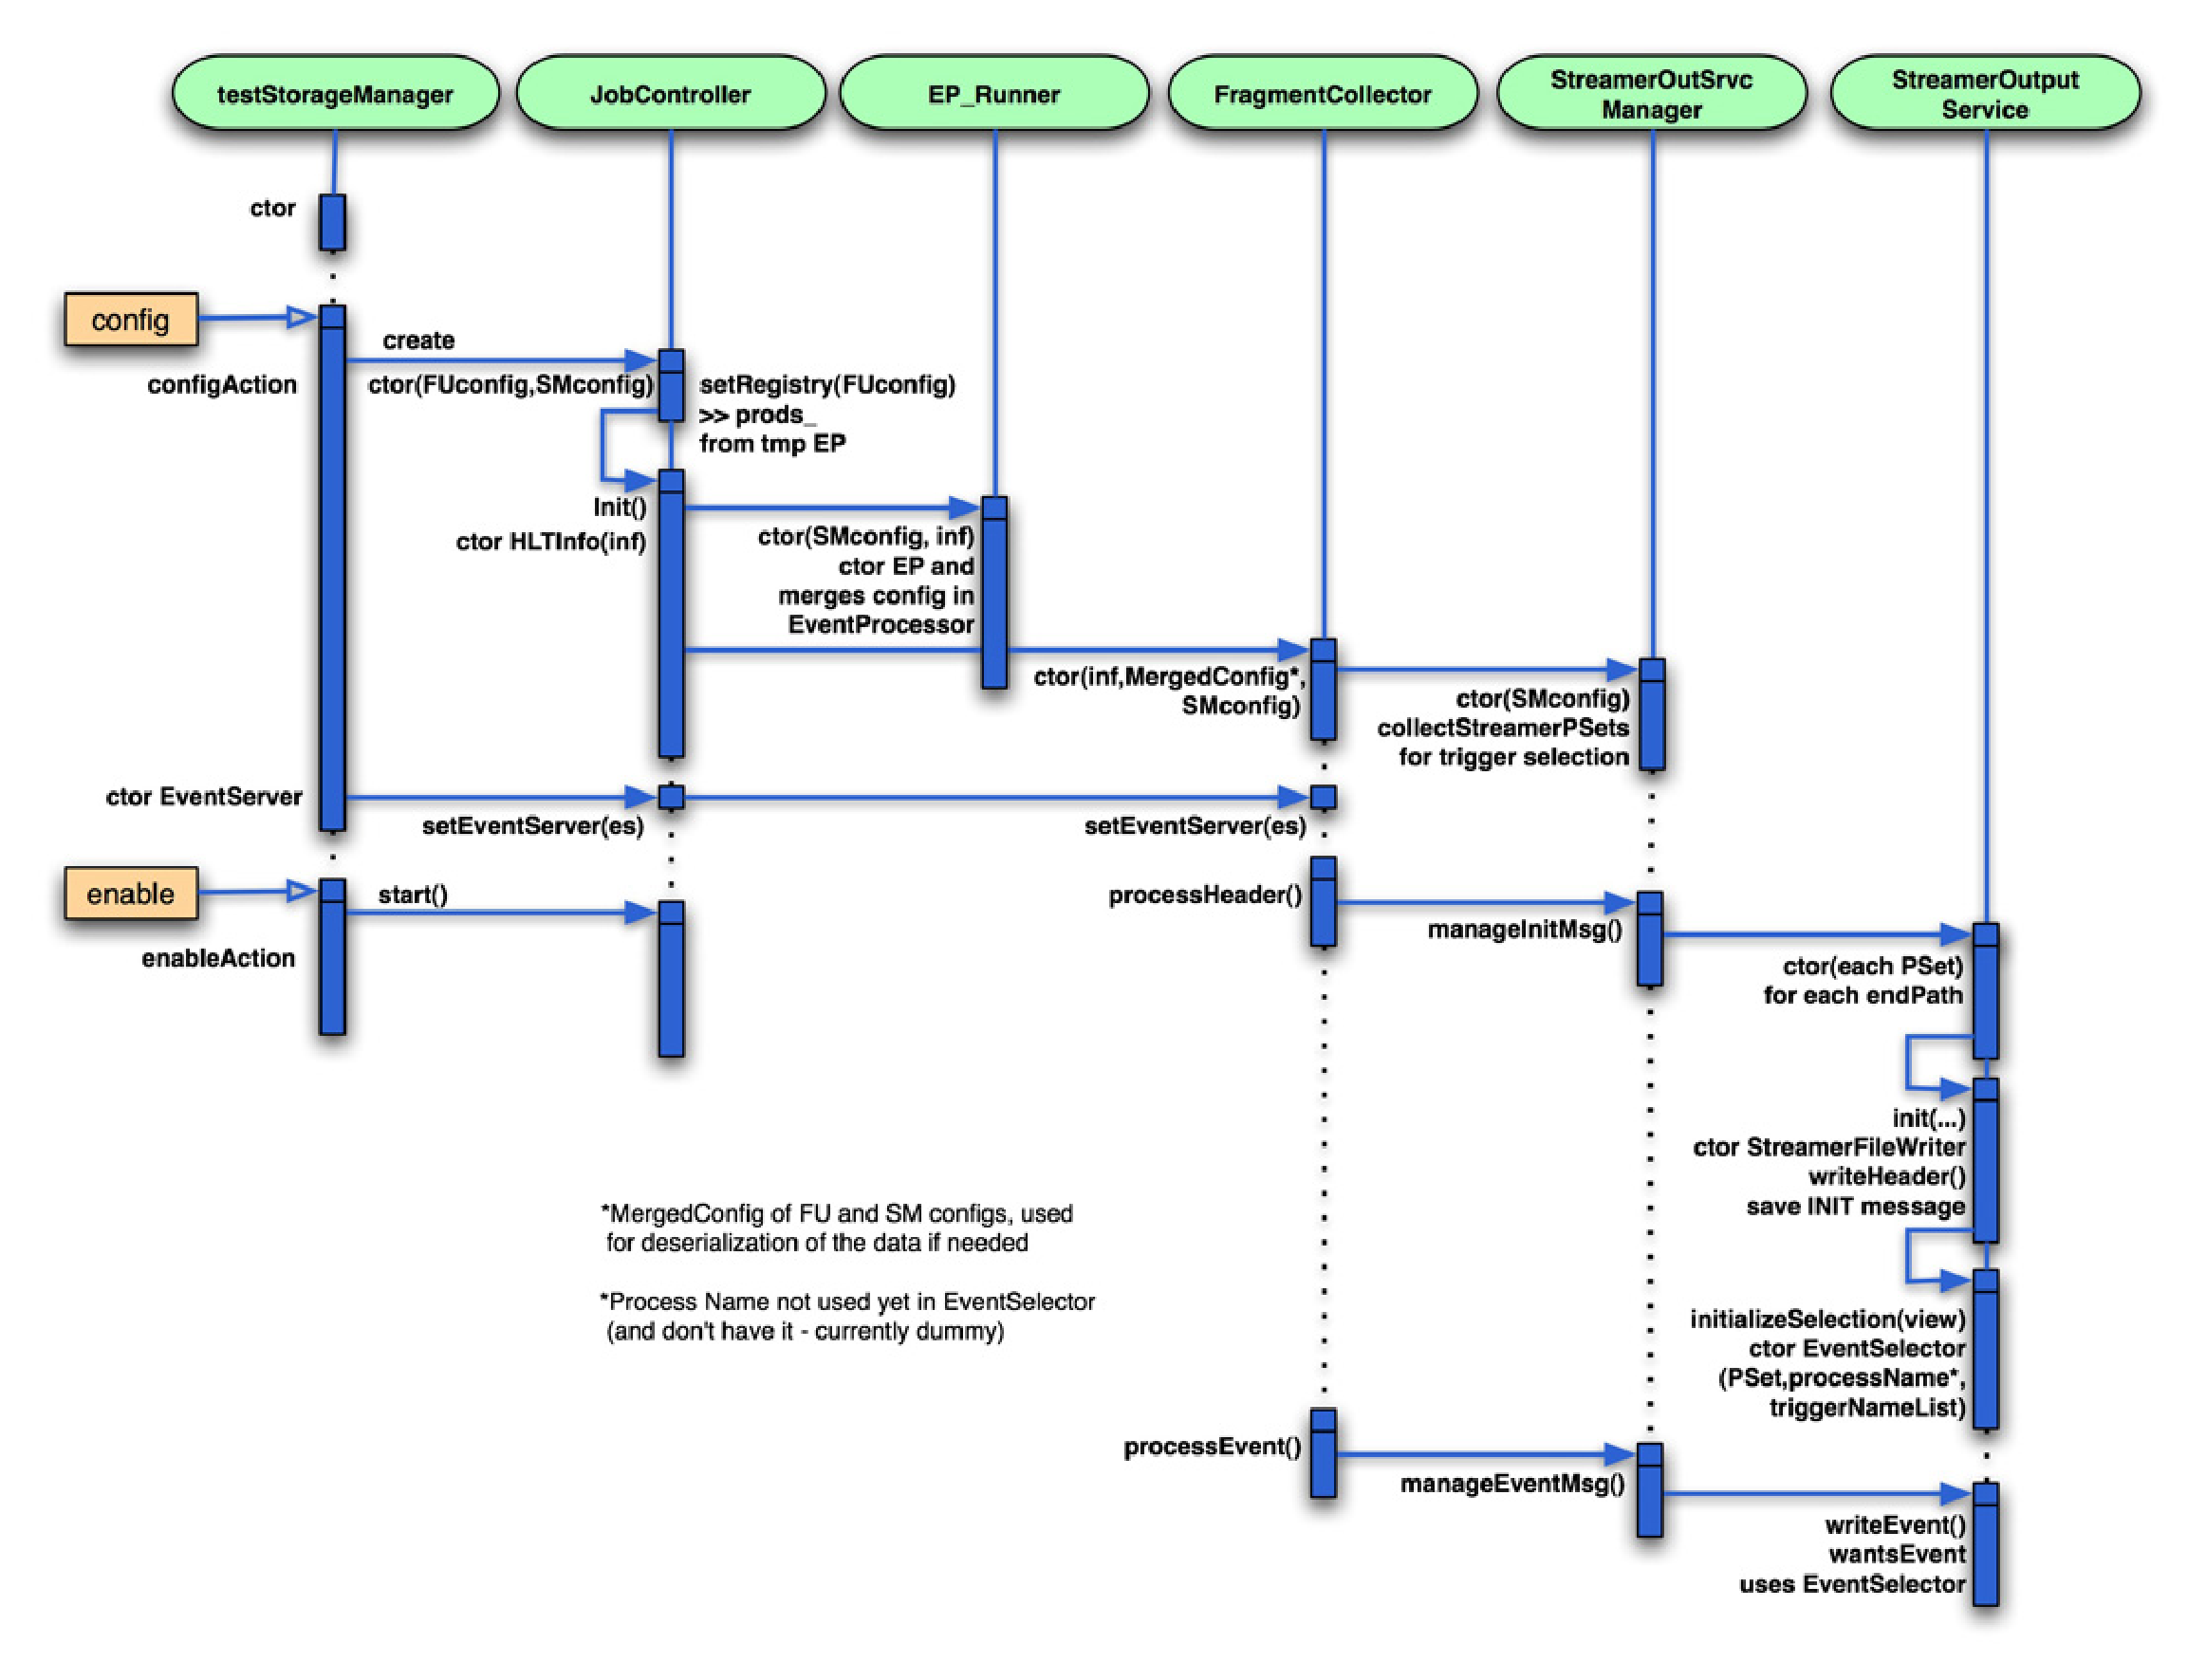
\includegraphics[width=5.5in]{SM_base_code2_prt-2.eps}
    \caption{Storage Manager configuration sequence.}
    \label{fig:base_SMCF_code}
  \end{center}
\end{figure}

\begin{figure}[hbtp]
  \begin{center}
    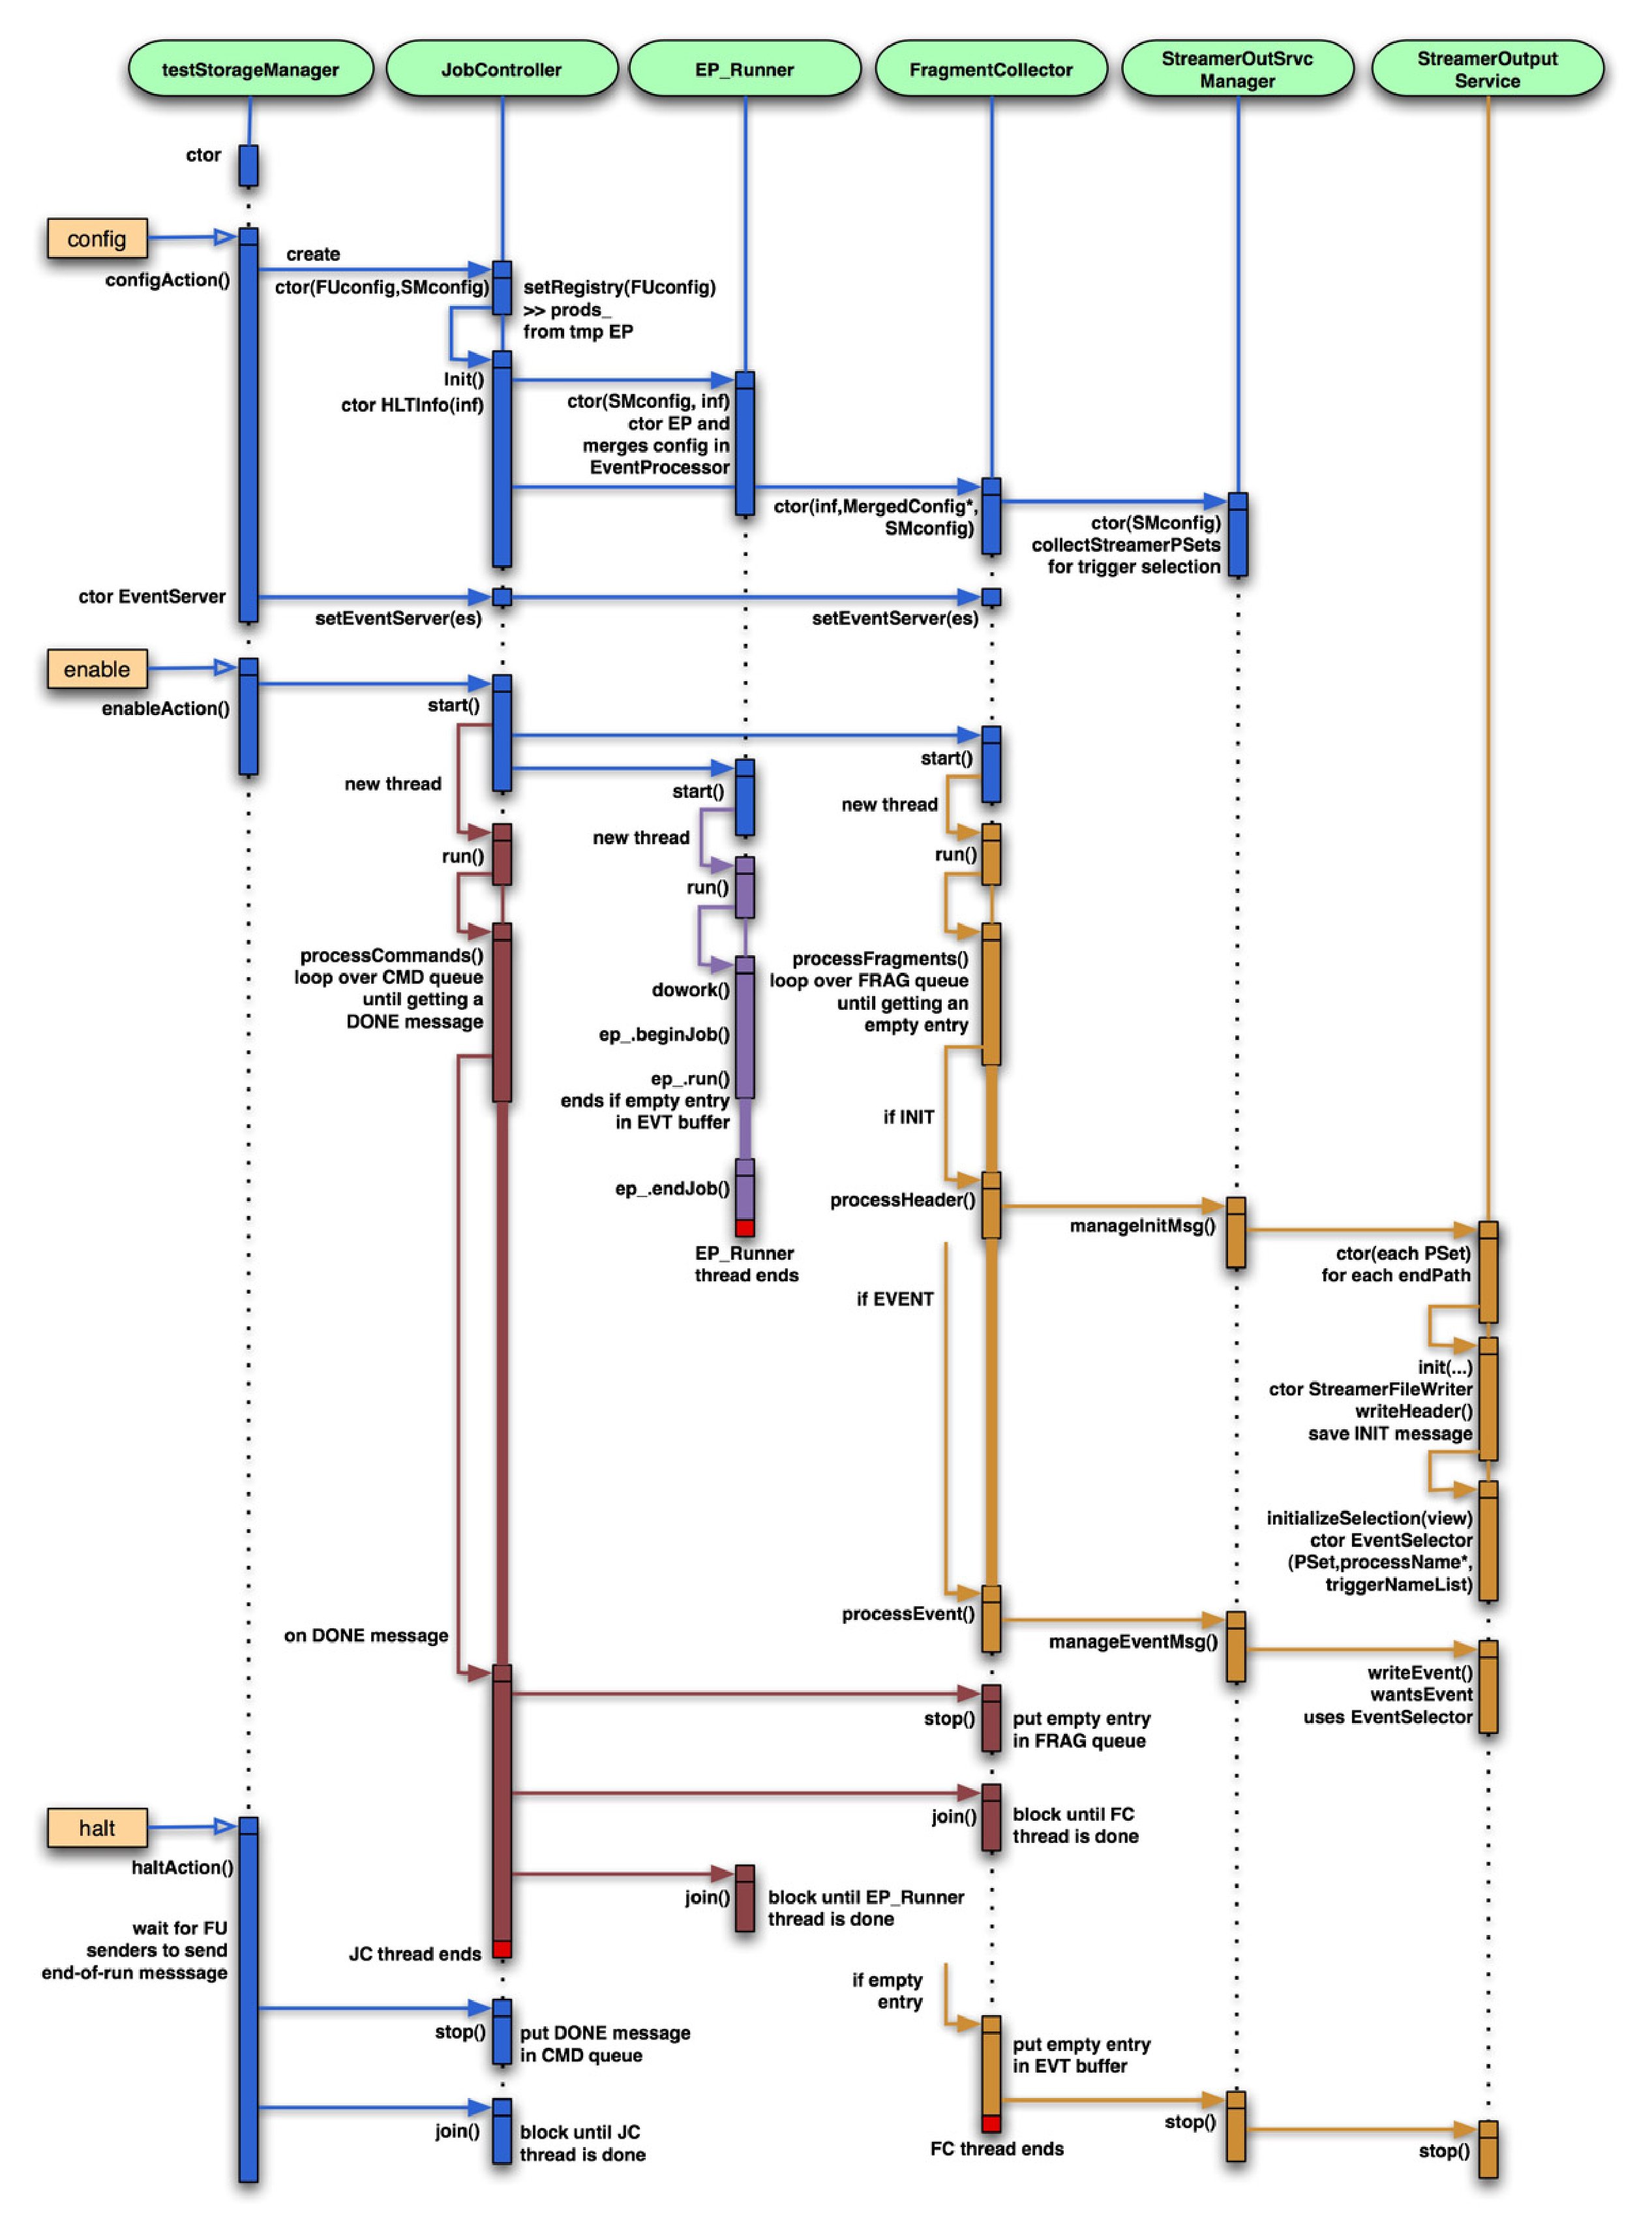
\includegraphics[width=6.0in]{SM_base_code3_prt-2.eps}
    \caption{Storage Manager sequence for prototype 2 code used in
    MTCC phase 2.}
    \label{fig:base_SMMTCC_code}
  \end{center}
\end{figure}

\begin{figure}[hbtp]
  \begin{center}
    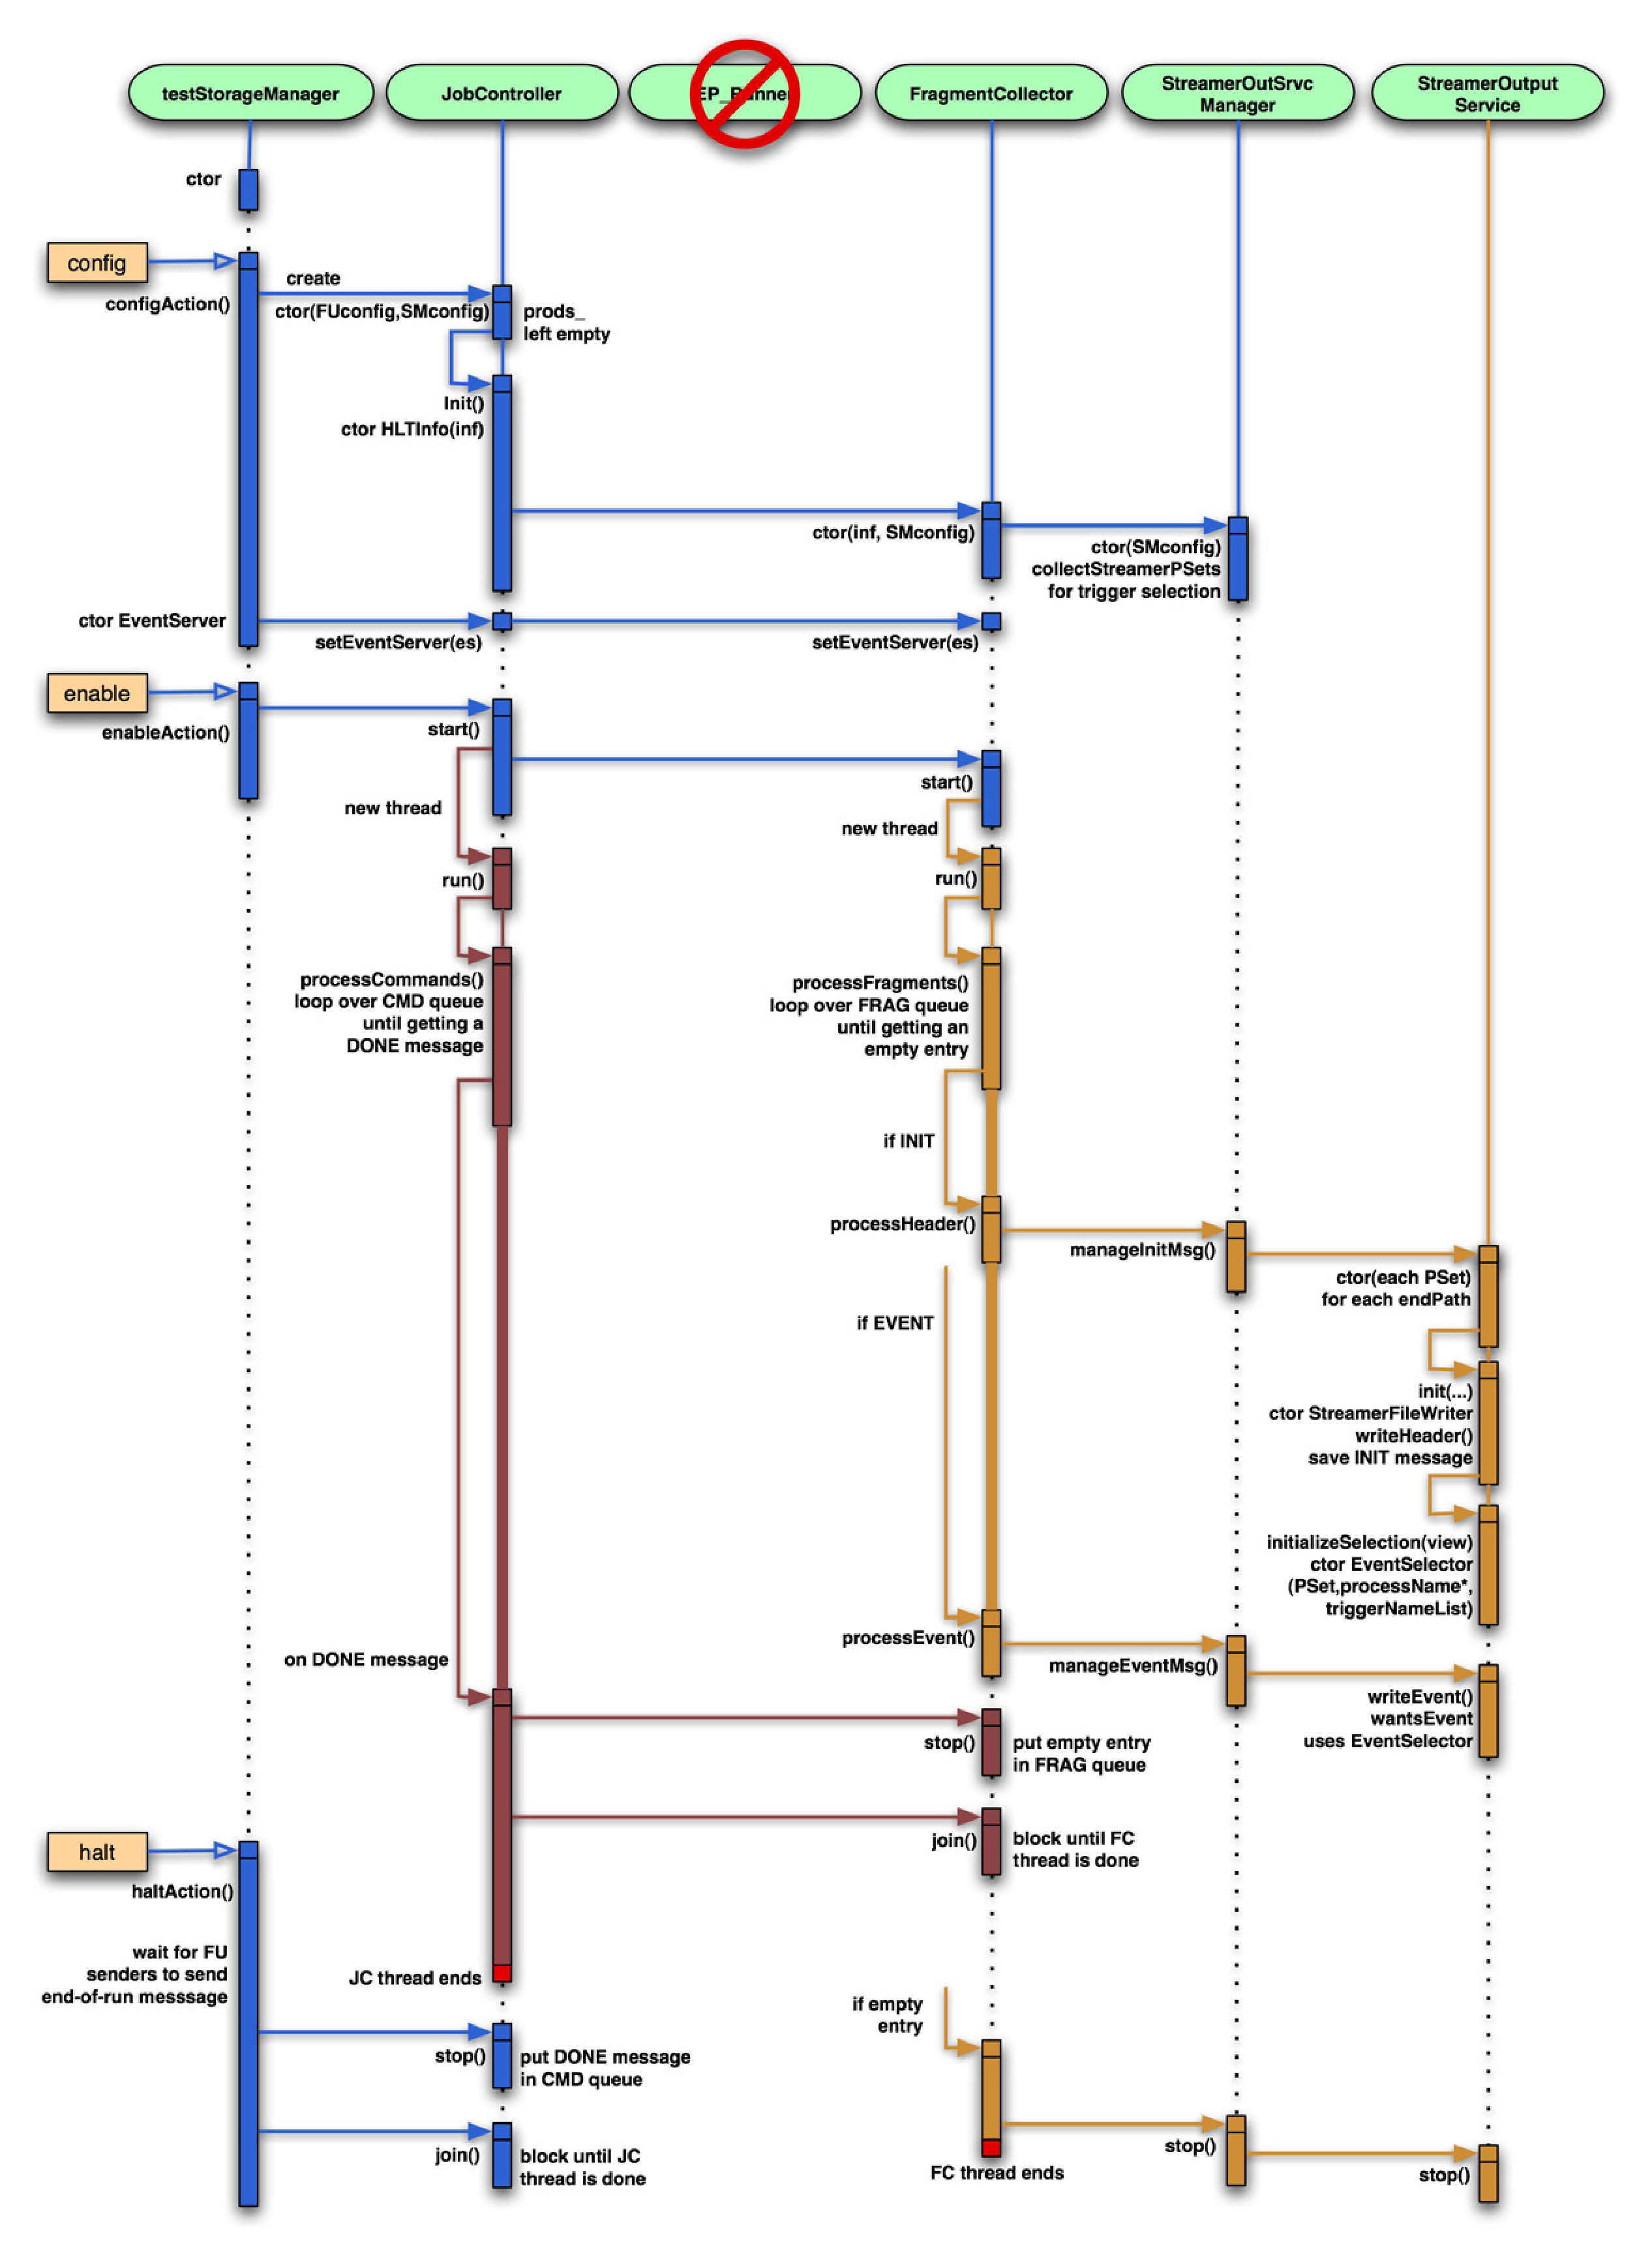
\includegraphics[width=6.0in]{SM_prd_code3_prt-2.eps}
    \caption{Storage Manager sequence for production code.}
    \label{fig:base_SMPRD_code}
  \end{center}
\end{figure}


\subsubsection{Possible Extension}

\begin{figure}[hbtp]
  \begin{center}
    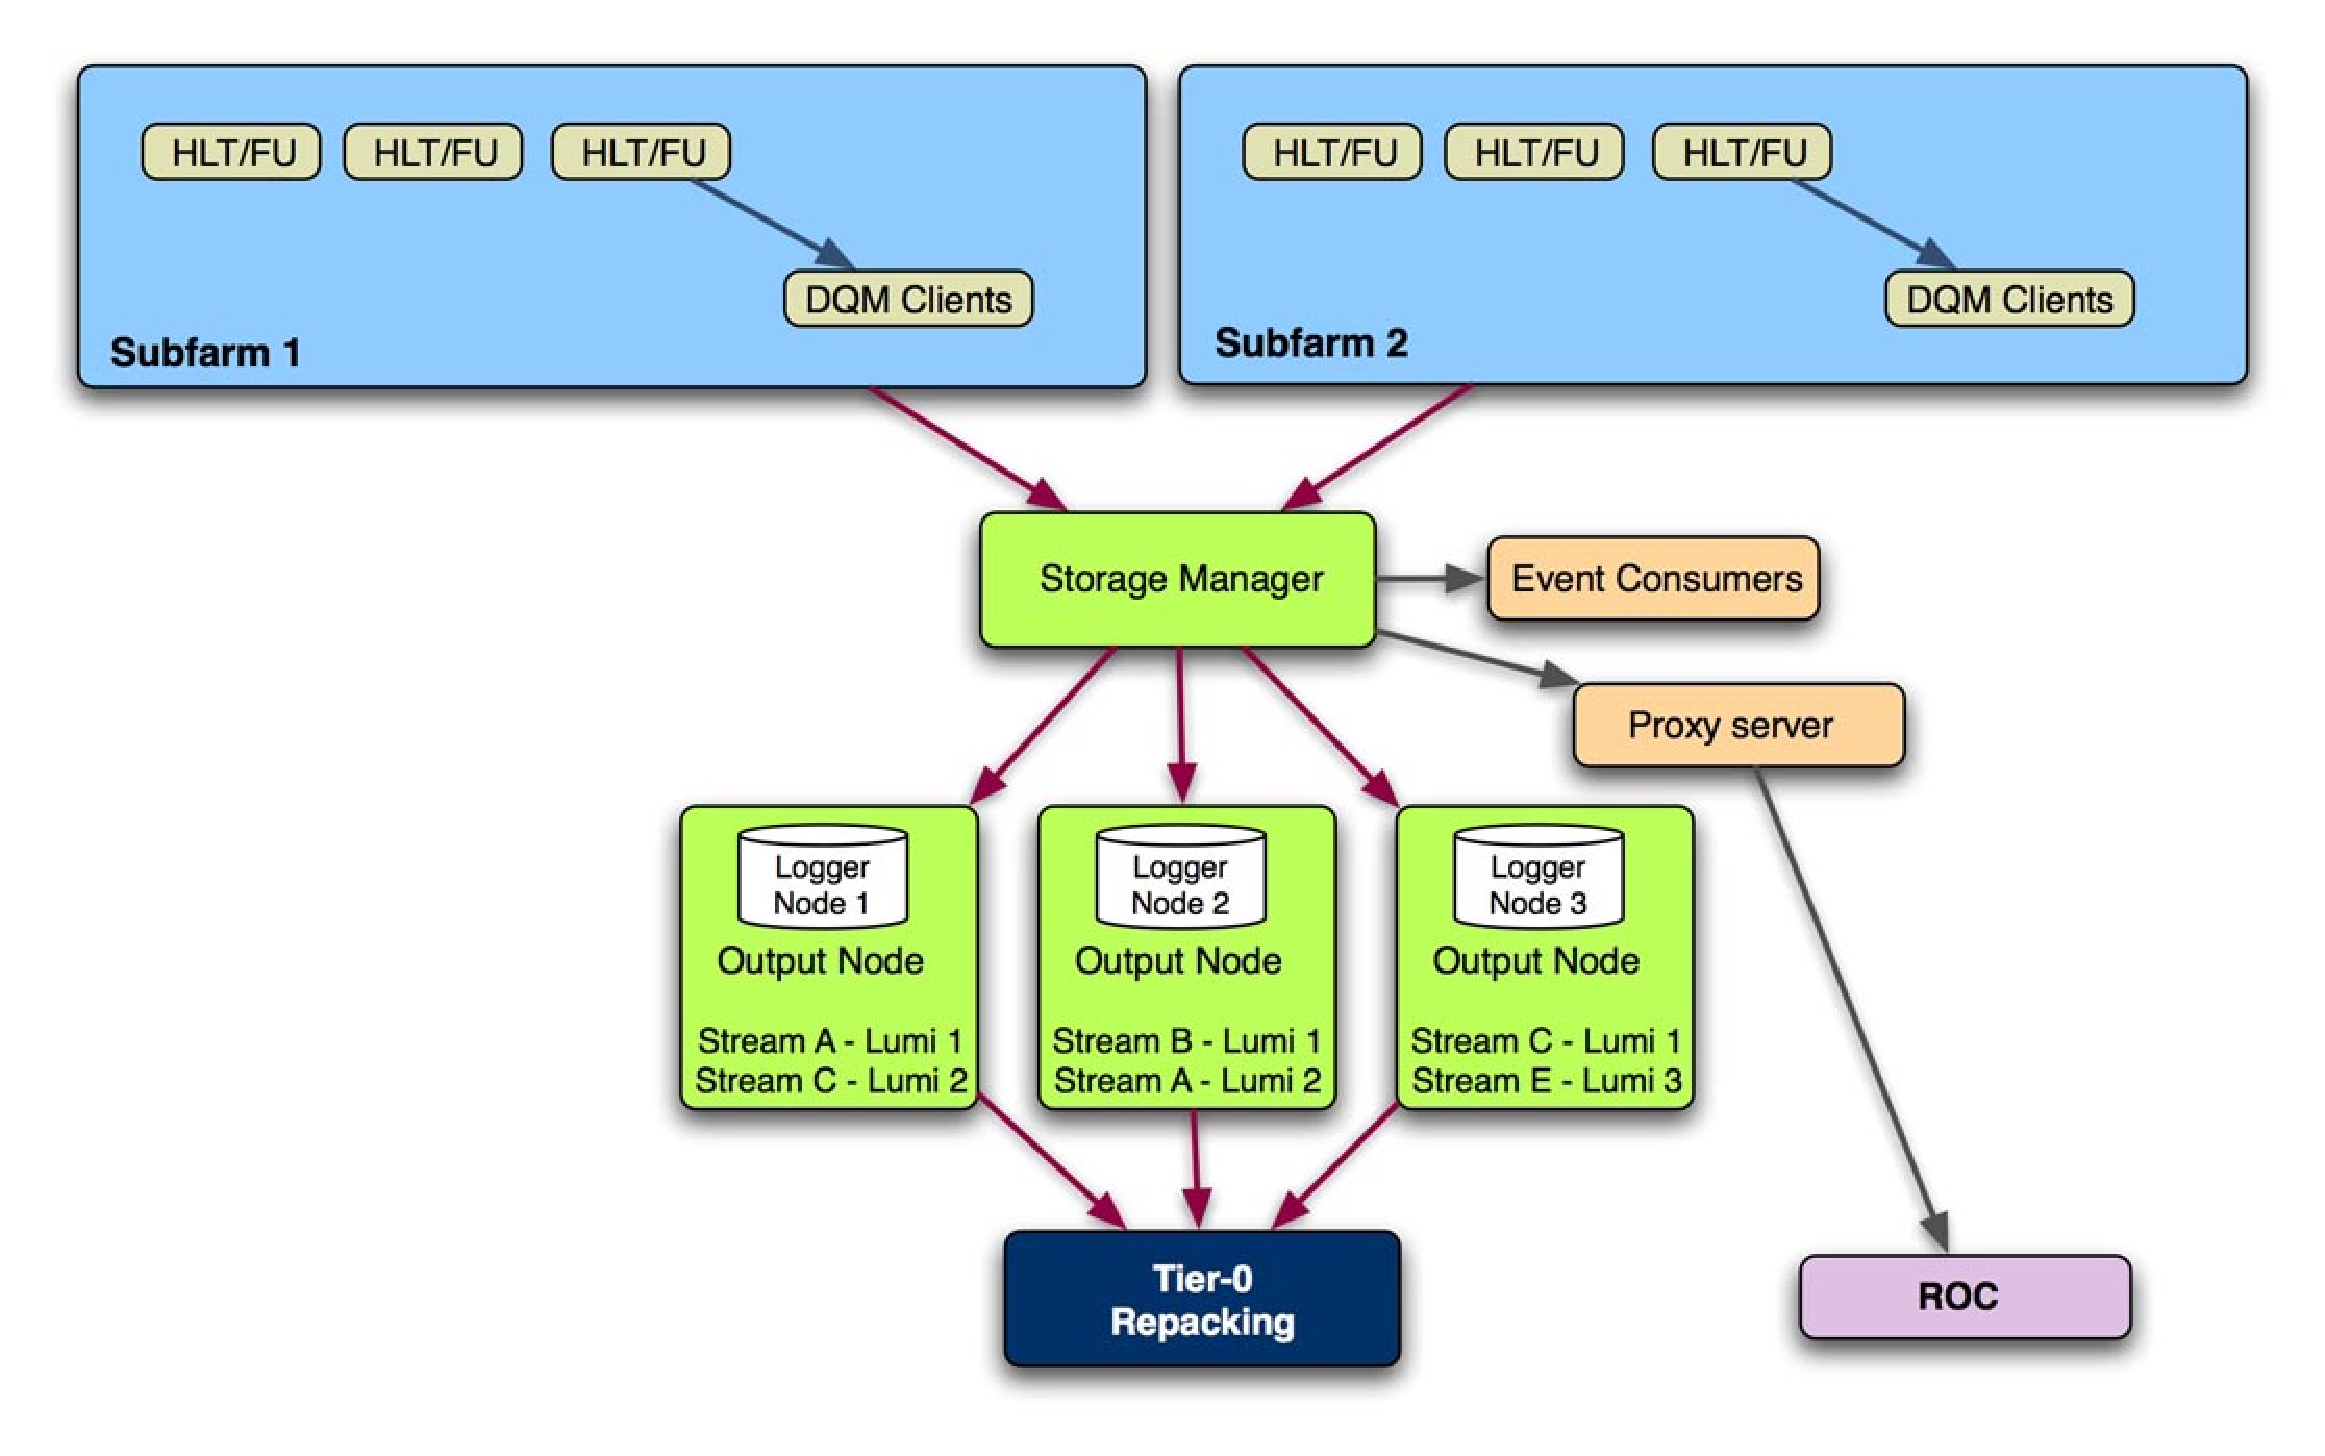
\includegraphics[width=5.5in]{SM_architecture_opt1.eps}
    \caption{Base design with integrated concatenator.}
    \label{fig:opt1_design}
  \end{center}
\end{figure}


\subsubsection{Future Design}

\begin{figure}[hbtp]
  \begin{center}
    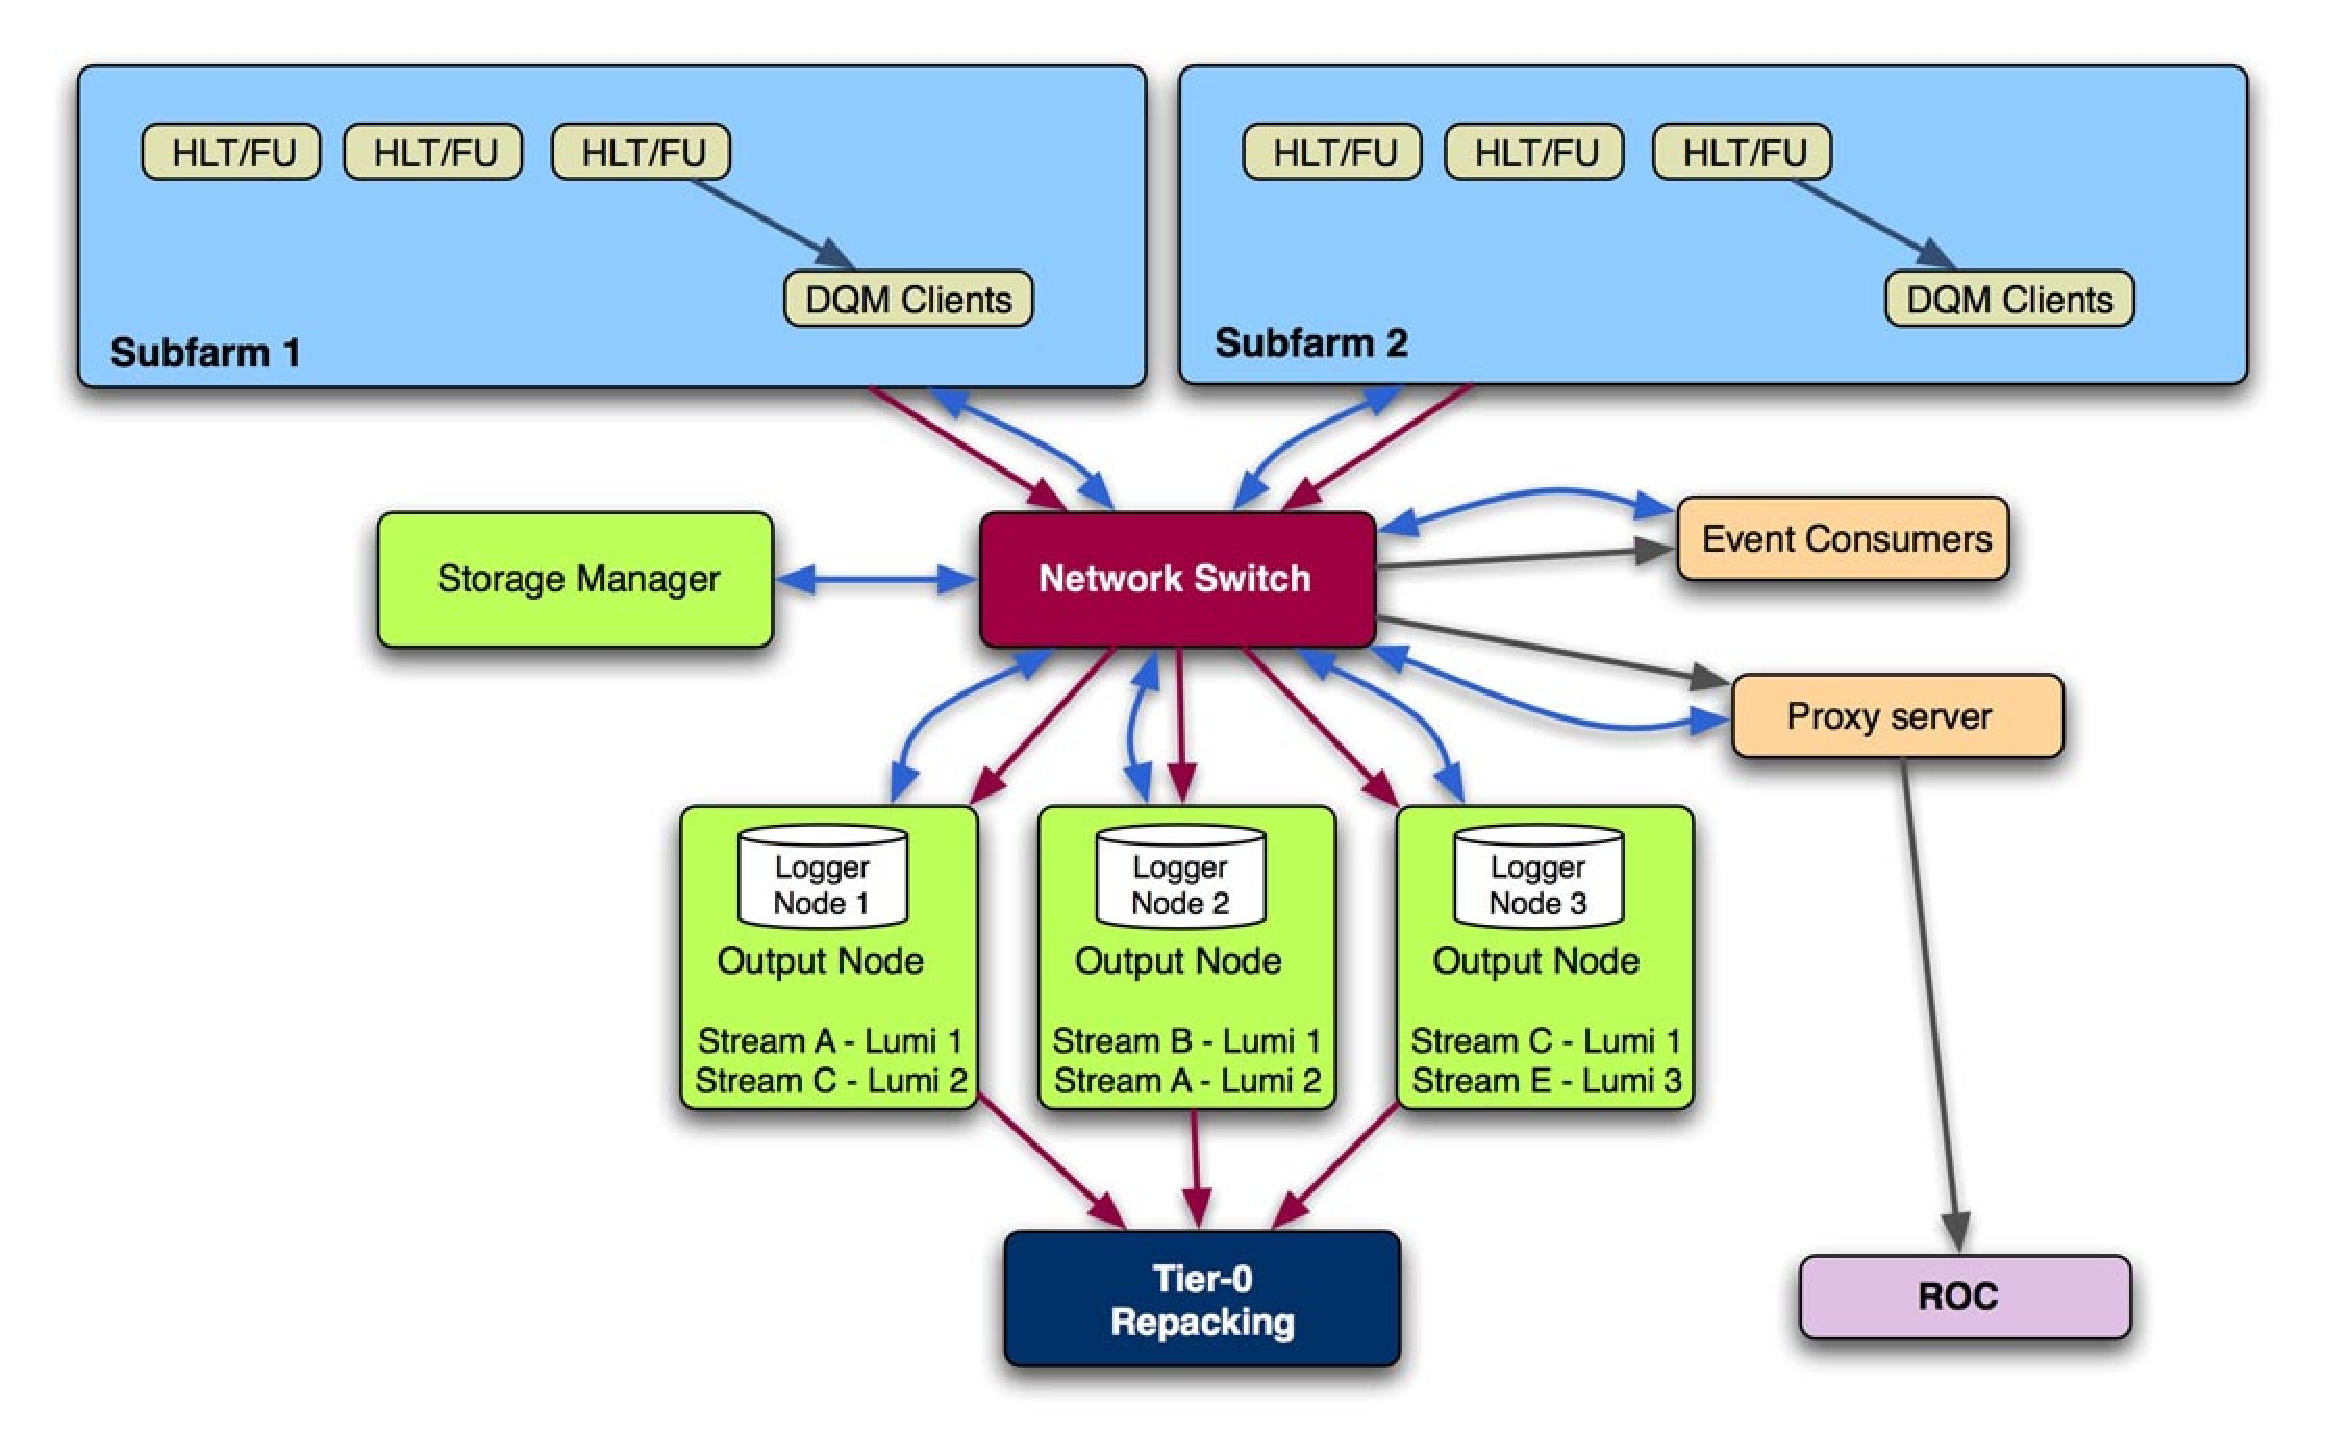
\includegraphics[width=5.5in]{SM_architecture_opt2.eps}
    \caption{Distributed Design.}
    \label{fig:opt2_design}
  \end{center}
\end{figure}

\subsubsection{Interaction with Tier-0}

\subsubsection{Interaction with Run Control}

Include DQM (hot disks, caches?)


\subsection{Communication and Output}

\subsubsection{Application protocol}

\flushleft{\bf Event Filter Unit (message formats)}

\flushleft{\bf Run Control}

\flushleft{\bf Tier-0}

\subsubsection{File formats}

Include index file

\subsection{Functions and Implementation}

\subsubsection{FU Output module}

\subsubsection{SM Input module and Collector}

\subsubsection{Internal event processing}

\subsubsection{SM Output module}

\subsubsection{Event Server Manager}

\subsubsection{Monitoring, Statistics and Book-keeping}


\section{External Functions and Interaction}

\subsection{Interaction with Databases}

\subsection{File and Disk Management Application}

Functions and design of the script(s).

\subsubsection{Conversion}

\subsubsection{Monitoring and Statistics}

Include trigger rates

% $Id: performance.tex,v 1.1 2008/05/26 20:05:29 gbauer Exp $



\section{Storage Manager Performance}

The Phase-I system, currently installed in Cessy, has
3 SATABeasts installed  with 10 Sata disks of 750~GB  and 116 of 1~TB.
These are currently configured in our baseline in groups of 10-disk RAID5 arrays 
(2 spare RAID disks per SATABeast), yielding an effective capacity of 105.75~TB storage
for the full system.
With the dual controllers, a single SATABeast is expected to be fundamentally 
limited to about 400 MB/s writing.

The HLT subfarms are connected via a FORCE10 switch through
two 2~GbE Silicom links (``rails'') per logger node.
Presently the DAQ system is being recabled for the full contingent of eight FORCE10 switches
such that each switch, corresponding to a DAQ ``slice,'' has connectivity with 
a single SM logger node.
Another layer of a pair of additional switches are being contemplated by the DAQ group
that would remove this restriction.
The Ethernet connection limits the theoretical wire-speed of data input
to a logger node to 250~MB/s.

Each logger node is connected to the Tier-0 switch with a single 2~GbE link.  

The 3-SATABeast Phase-I system was designed to be able to provide a throughput of about 1~GB/s,
but it falls short of the design of 250~TB capacity. 
This requires an expansion of the system, which is discussed in Section~\ref{sec:SMexpansion}.
Because each SATABeast will collect the data from two DAQ slices, and the slice structure
is a simple replication of parallel structures, a single SATABeast fed by two logger nodes
is the atomic unit for projecting throughput performance---although we usually quote
results on a per-node basis, test numbers are
obtained using two nodes each accessing a separate disk array and controller per node.
We use this model in our performance studies and extrapolation to that of the full system.

The nominal setup for our system tests include the following features, unless stated
otherwise:
\begin{itemize}
  \item SLC4 Linux installation on logger nodes,
  \item 2 logger nodes accessing separate ten-physical-disk arrays on the same SATABeast,
  \item Each logger node has control of two arrays, and alternates the file writing,
between these two arrays as luminosity sections are incremented,
  \item 128k SATABeast stripe size (maximum possible),
  \item RAID5 disk redundancy,
  \item xfs file system on the SATABeasts,
  \item Single output stream,
  \item $\sim$1 MB event size, and
  \item 1 GB data file size. 
\end{itemize}
Our tests can be categorized in terms of subcomponent capability and full system tests.
Subcomponent tests include:
\begin{itemize}
  \item {\bf Ethernet Input on Logger Nodes:} The Ethernet throughputs have been tested for two cases.
First, we have set-up the full DAQ readout chain but flagged all the data from FUs to the SM
to be transferred but {\it not} actually written out. In this case a 1-rail SM sinks about 110 MB/s,
and a 2-rail SM takes in 220 MB/s.
Similarly, the single logger-node link to Tier-0 for simple file transfers (with no other activity)
also saturates  at about  110 MB/s.
  \item {\bf Direct Logger Node Write/Read to a SATABeast:} To gauge the write performance 
from a logger node to a SATABeast 3 GB files were generated by \verb+dd+ (64k block size)
and written to a  SATABeast disk array. Read tests were done with 1 GB files. 
Early tests with few disks provided rather low rates, but
later we settled on 10-disk arrays as a compromise configuration. 
We obtained the following results:
%\begin{table}[h]
\begin{center}
\begin{tabular}{c|c|c|c}
\# nodes   & \# Arrays & Write Only (MB/s) & Read Only (MB/s) \\ \hline
1          &     1     &     198           &    211\\
1          &     2     &     198           &    200\\
2          &     2     &     377           &    383\\ \hline
\end{tabular}
\label{tab:ddrates}
\end{center}
%\end{table}
With two logger nodes we have driven the SATABeast near the expected 400 MB/s maximum.
Similar performance was seen with \verb+dc_bench+.

The choice of 10-disk arrays is, as much as anything, almost a forced choice
given that that the SATABeast is limited to 42 disks and at least 2 disk spares
seems to be a minimum choice, and one would like an even number of arrays.
In terms of \verb+dd+ write rates, 10 disks turns out to be a reasonable choice as 
write performance is almost saturated at 10 disks:
\begin{center}
\begin{tabular}{l|c|c|c|c|c} \hline
\# Disks:      &   6    &   7    & 8    & 10   &   13\\ \hline
Rate (MB/s):   & 160    & 174    & 180  & 198  &  200\\ \hline
\end{tabular}
\label{tab:ddrates2}
\end{center}
  \item {\bf Data Transfers to Tier-0:} We have tested reading data files from
a  SATABeast via logger nodes and sending them out through a single  2~GbE link
to Tier-0.
Dedicated read-only from the SATABeast, and using the standard \verb+CopyWorker+
transfer scripts, saturates the Ethernet at about 100 MB/s per logger node.
\end{itemize}

We put all the pieces together in full system tests, 
which run the standard SM executables and employ the full DAQ chain.
We do not have front-end detector readouts available for our tests, 
but the component that reads the front ends and interfaces them to the event builder,
the Front-end Readout Link (FRL), has a feature whereby it can internally generate
data to simulate detector payloads.
Our DAQ chain begins with  one or two crates of FRL's generating data
sending  these event fragments to built by the normal chain of PC's serving
as Readout Units (RU's) to collect superfragments,
Builder Units (BU's) to build complete events,
then feed them to Filter Units (FUs), and finally
pass the events to the SM for recording over two Ethernet rails.
The filter algorithm of the FU has data  compression turned off and 
the event size was padded in the FU with dummy arrays to make it about 1 MB.

The operation of the SM consists of a series of stages which can be
functionally subdivided as:
\begin{enumerate}
  \item SM receiving and handling events from the FU  
  \item SM writing events to disk (each logger node alternates between writing to two of its own  arrays)
  \item For each file written: database operations for file bookkeeping and for the transfer system 
        are done by the SM executable
  \item Actual DB operations and transfer of files to Tier-0 are done by independent processes
        (not by the SM executable) 

\end{enumerate}
The throughput rates measured for various permutations of these processes being
active or not in full DAQ running  are (in MB/s):
\begin{center}
\begin{tabular}{c|c|c|c|c|c} 
2. Write Files & 3. DB actions & 4.Send   & SM      & Tier-0     & Per SATABeast \\ 
               &               &to Tier-0 &  ~Rate~   &Rate  & Controller Rates \\ \hline
   NO       &   NO       &    NO          &       220      &   --- &   ---       \\
 {\bf YES}  &   NO       &    NO          &       180      &   --- &   180       \\
 {\bf YES}  &  {\bf YES} &    NO          &       144      &   --- &   144       \\
 {\bf YES}  &   NO       &   {\bf YES}    &       150      &    50 &   150$+$50  \\
 {\bf YES}  &  {\bf YES} &   {\bf YES}    &       150      &    50 &   150$+$50  \\
\end{tabular}
\label{tab:rates}
\end{center}
These rates are quoted on  a {\bf per logger node} basis, although the measurements
were actually performed with two logger nodes each feeding separate arrays 
on a single SATABeast, and thus a  SATABeast itself has a total rate of 300$+$100 MB/s.

It is interesting that there is a noticeable, and equal,  penalty for DB actions
and for transfers to Tier-0, but one seems to ``shadow'' the other.
Also note that these test were done with the old method of DB access, which was managed 
by processes initiated by the SM executable. We have been  restructuring this whereby
the DB access is entirely decoupled from the SM executable (see Section \ref{sec:fpt0}).
This may reduce the overhead delays in the SM from DB access.
We do not, however, count any performance improvement from this change.
This example highlights the fact that other fine-tuning of the system may be possible,
and profitable, for improving SM performance, but we note that this does not appear 
to be actually necessary for the SM to meet our original goals.

A further teasing apart of the effects on throughput is seen in an early
test with two SM nodes writing to two arrays on a SATABeast, of 6 and 7 disks respectively,
that gave a rate of about 140 MB/s writing 1 GB files (no reads).
When each node was reconfigured to write the output in a {\it single} file of unlimited
size the rate increased to about  150 MB/s.

Questions about CPU load can only be fully addressed with all functionality
in place, including the eventual DQM load.
A rough look at the \verb+top+ load when running the full DAQ chain and
transfers to Tier-0 indicate the CPU is occupied $\sim$15-30\% by the system plus ``users,''
$\sim$20-50\% in I/O wait, and $\sim$20-80\% idle.
No problem is apparent at this point.
Heavier demands from additional tasks could change this picture, 
especially motivating an expansion of PC memory.

A variety of miscellaneous issues were investigated with respect to throughput rates:
\begin{itemize}
  \item {\bf File Systems:}
Our initial choice for the file system was xfs.
However, during heavy loading with \verb+dd+ tests, and relatively rare incidents 
in full DAQ running,
we observed the logger nodes crashing (log messages indicated paging problems).
We tested a Linux kernel build under SLC5, and did not observe this problem.
However, operating with what is at this point non-standard software is not 
viewed as a very practical option.
We also configured the SATABeast file system under ext3, and again did not observe
this problem.
In fact, most of the May Global Run (CRUZET-1) was run  with  ext3
without any SM incidents.
We still need to  be sensitive to possible negative impacts of choosing  ext3 over xfs,
but so far we have not uncovered any downside with running  ext3,
and we have now adopted it as our default system.

  \item {\bf Multiple Output Streams:}
We have done a preliminary test running the full DAQ chain to the SM with 
up to 5 output streams so far.
Interestingly the throughput performance showed a small increase 
in rate to 192 MB/s (compared to the benchmark of 180 MB/s).
When running with even more streams we ran into reliability problems
with the xfs file system, as discussed in the previous bullet.
These tests need to be extended with ext3, but indications so far are
that multistreaming is not an issue.

 \item {\bf Large Number of Socket Connections:}
As a practical matter the SM is so far usually run with either a small number of FU's 
or  low throughput, and thus  one has  not been sensitive to the impact on performance 
of a SM node having to manage a large number of socket connections.
For 2008 LHC running the DAQ system expects to be running about 720 FU's---one
\verb+EventBroker+ (i.e. one socket connection to the SM) each.
With a 16-SATABeast system each logger node would support 45 FUs,
and any eventual system doubling would only push this 
to 90 FUs per logger.\footnote{Because of the finite rack space available, 
the DAQ group is significantly constrained that future increases of the filter farm take 
the form of larger numbers  CPU cores per FU rather than proliferating physical boxes.
This implies that even dramatic increases in CPU power of the filter farm
should not have a large effect on the connection load of the logger nodes.
Although, future upgrades with more rails is a possibility, but the capability
of the logger nodes would also presumably be improved.}
We ran a large connection test by feeding the output of 100 FUs into
a single SM (ext3 file system, no DB actions, and no Tier-0 transfers) and
achieved the usual write rate of 180 MB/sec.
An even larger system of 300 FUs showed only a modest drop to 150 MB/s.
\end{itemize}

Our essential conclusion is that while there may be worthwhile optimizations 
of the system, these results with one SM ``leg'' demonstrate that we are on track
to meet our performance goals even with the {\it existing}
state of the hardware and software.





\pagebreak
 \section{User Manual}
 
 

%\section{Reference example}
%
%References should be placed at the end of the note 
%(see example \cite{NOTE000}).
%
%\begin{thebibliography}{9}
%  \bibitem {NOTE000} {\bf CMS Note 2005/000},
%    X.Somebody et al.,
%    {\em "CMS Note Template"}.
%\end{thebibliography}
 
%------------------------------------------------------------------------------

\pagebreak
\section{Glossary}

 

\end{document}
